\documentclass[a4paper, 12pt, titlepage, legno]{article}
\usepackage[english]{babel}
\usepackage[a4paper, inner=1.25in, outer=1.25in, top=1.25in, bottom = 1.25in]{geometry}
\usepackage{amsmath}
\usepackage{amssymb}
\usepackage{amsthm}
\usepackage{wasysym}
\usepackage{booktabs}
\usepackage{array}
\usepackage{marvosym}
\usepackage{graphicx}

\begin{document}
\tableofcontents

\newpage

\section{Boog}
\begin{equation}
C H_{3}+N O_{2}^{-} \rightleftarrows Ag\left(S O_{4}\right)_{3}
\end{equation}

\begin{equation}
x=\frac{-b \pm \sqrt{\left(b^{2}-4 a c\right)}}{2 a}
\end{equation}

\section{oog}
\begin{figure}[ht!]
\centering
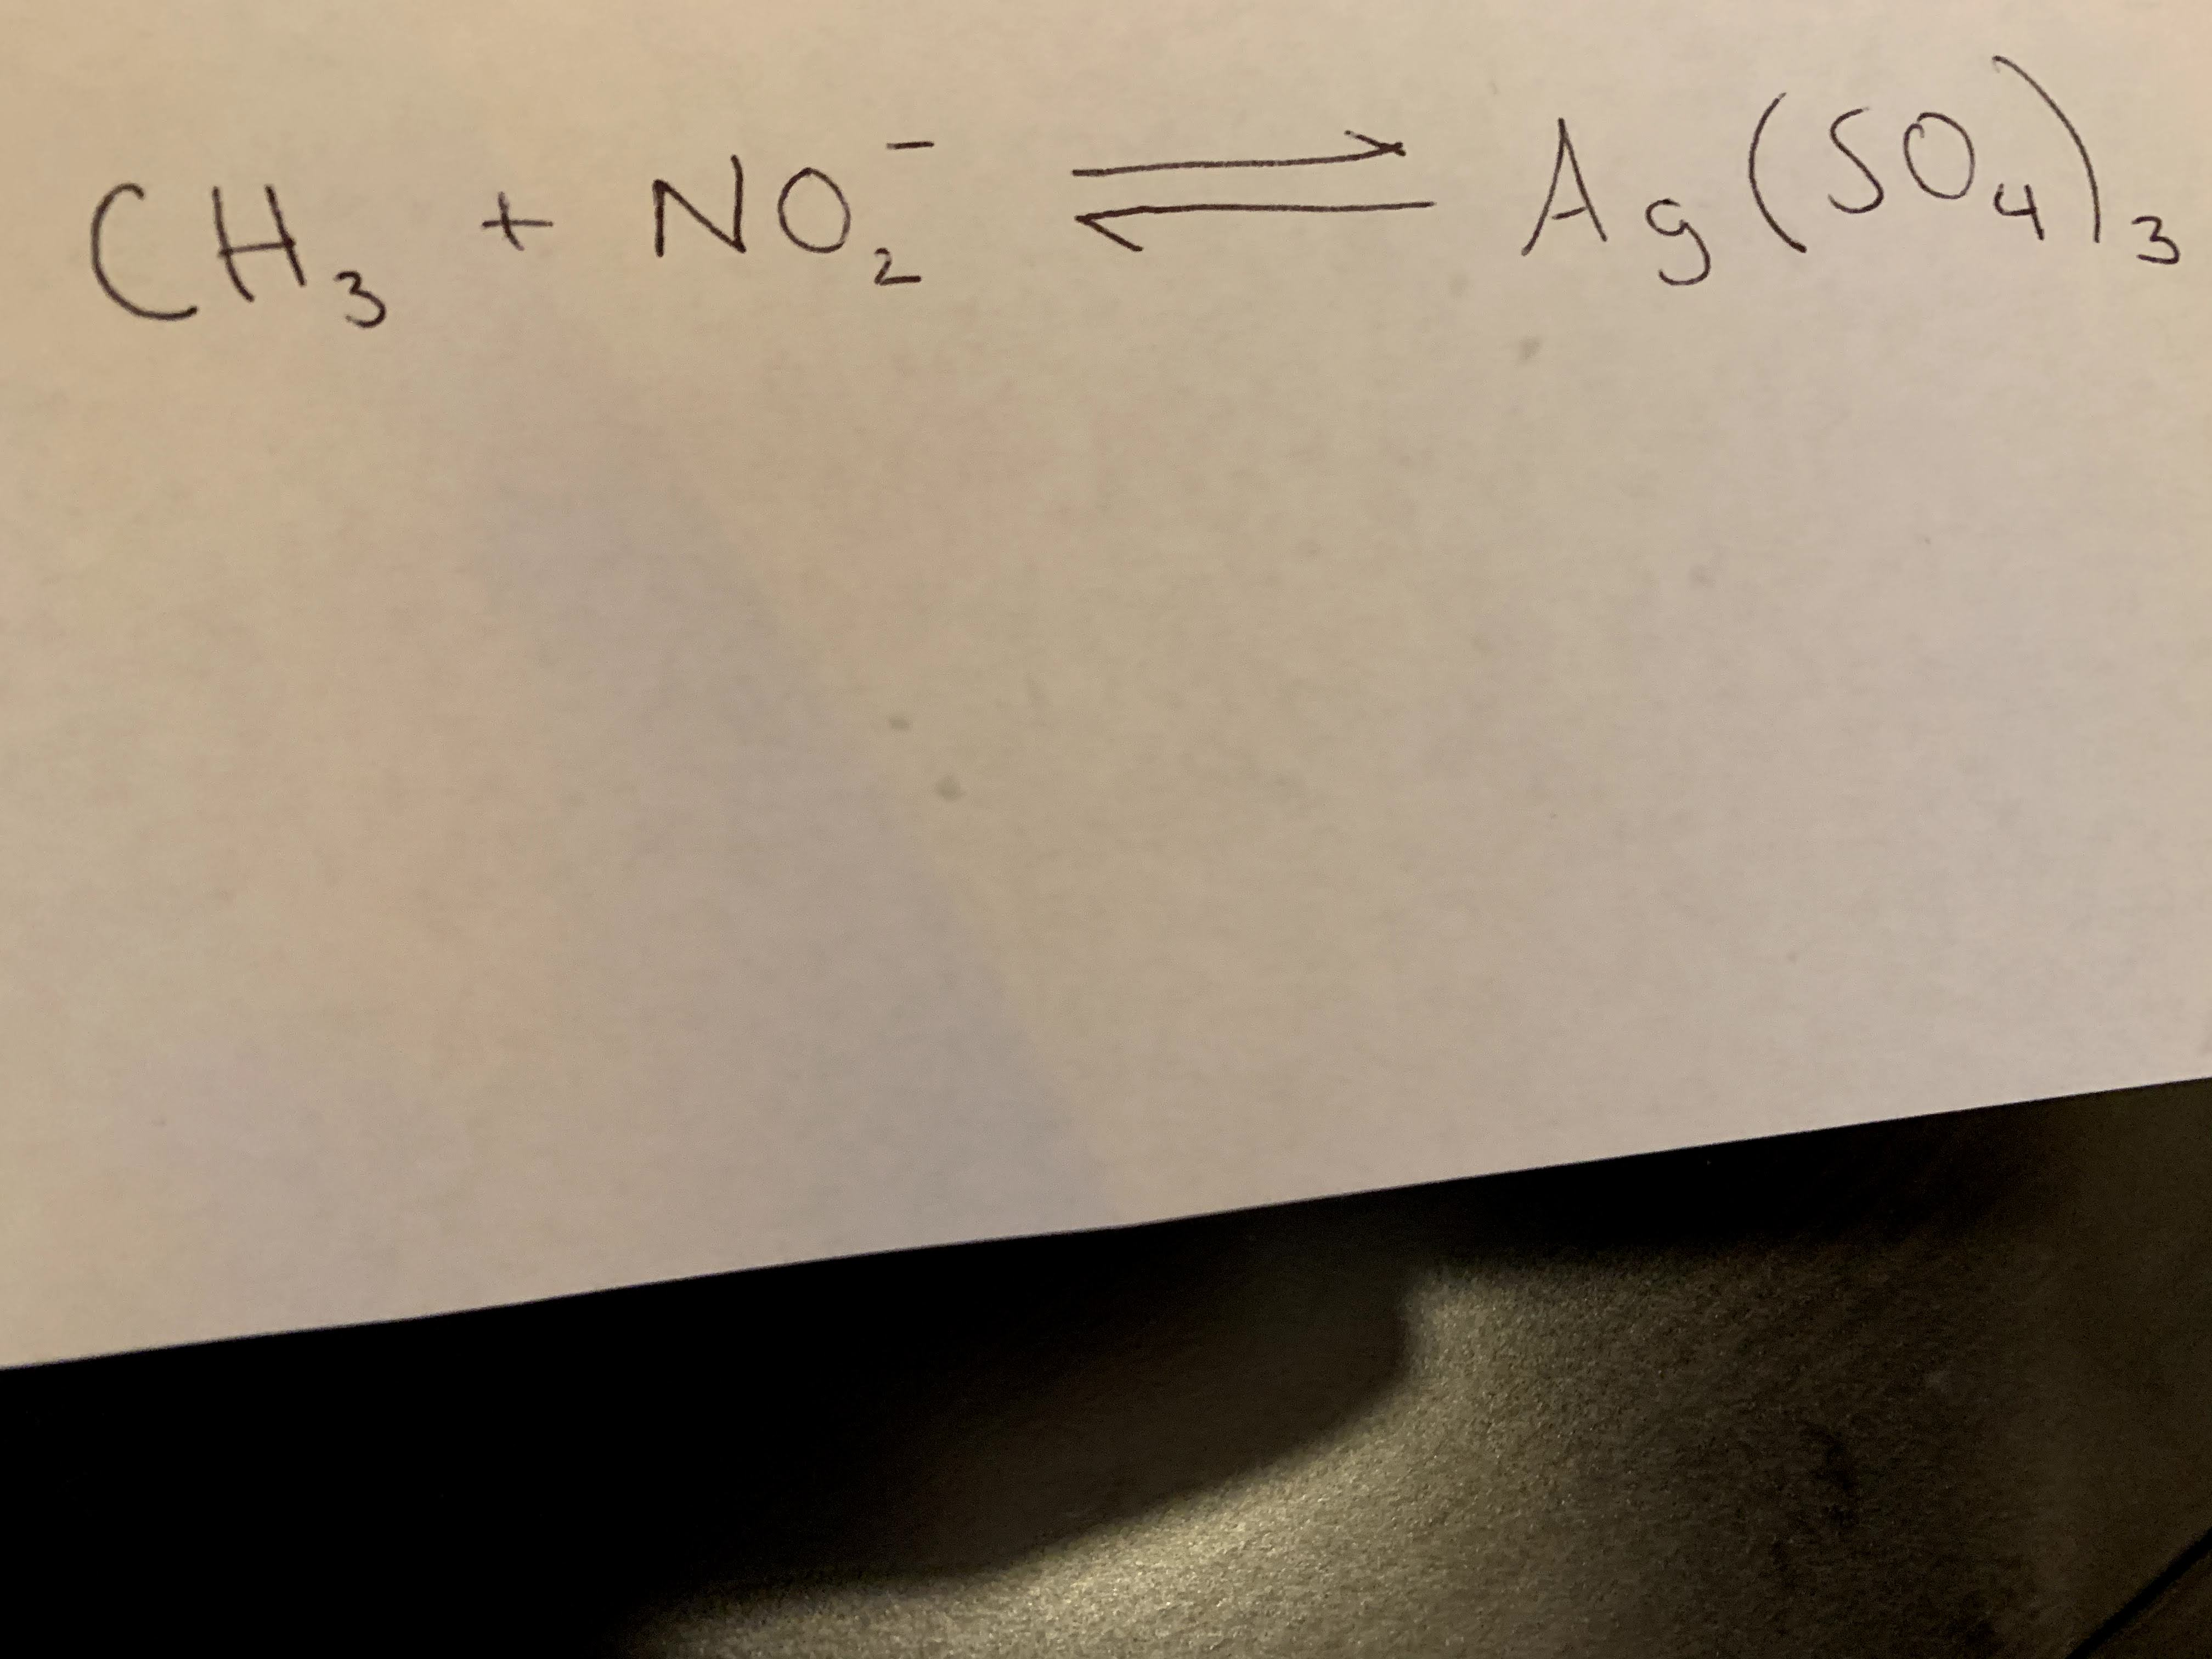
\includegraphics[width=90mm]{./imgs/IMG_8642.jpg}
\end{figure}

\end{document}